\documentclass[english]{article}

\usepackage{babel}
\usepackage{graphicx}
\usepackage{times}
\usepackage{pifont}
\usepackage[margin=1in]{geometry}
\usepackage{eurosym}
\usepackage{fancyhdr}
\usepackage[hidelinks]{hyperref}
\usepackage{listings}
\usepackage{color}
\usepackage{float}
\usepackage{listings}
\usepackage{caption}
\usepackage{subcaption}

\pagestyle{fancy}
\fancyhf{}


%HEADER
%**************************************************************************************
\pagestyle{fancy}
\fancyhf{}
%**************************************************************************************
\lhead{Timers as counters}		 	 
\rhead{Basics of Microprocessor technology} 
\lfoot{EFA12SF}
\cfoot{\thepage}
\rfoot{Alexey Tukalo}
%**************************************************************************************

\date{}
\setlength\parindent{0pt}

\begin{document}

\title{\vspace{2in}Timers as counters\\
\small for Basics of Microprocessor technology\\
\vspace{0.5in}
\includegraphics{savonia.jpg}}

\nopagebreak
\maketitle


\vspace{3in}

\author{
\begin{flushright}
Alexey Tukalo,\\
EFA12SF,\\
Information Technology,\\
Savonia University of Applied Sciences
\end{flushright}
}

\date{\today}
\thispagestyle{empty}

\newpage
\setcounter{page}{1}
\setcounter{tocdepth}{2}
\tableofcontents

\newpage

%MAIN CONTENT ******************************************************************************************************************

\section{The main features of counter circuits}
There are two types of counters in ATmega boards.
\subsection{8-bit Timer/Counter}
\begin{itemize}
\item Two Independent Output Compare Units
\item Double Buffered Output Compare Registers
\item Clear Timer on Compare Match (Auto Reload)
\item Glitch Free, Phase Correct Pulse Width Modulator (PWM)
\item Variable PWM Period
\item Frequency Generator
\item Three Independent Interrupt Sources (TOV0, OCF0A, and OCF0
\end{itemize}

8-bit Timer/Counter module is used for accurate event management and wave generation. It has two independent Output Compare Units, and with Phase Correct Pulse Width Modulator support.
\subsection{16-bit Timer/Counter}
\begin{itemize}
\item True 16-bit Design (that is, allows 16-bit PWM)
\item Three independent Output Compare Units
\item Double Buffered Output Compare Registers
\item One Input Capture Unit
\item Input Capture Noise Canceler
\item Clear Timer on Compare Match (Auto Reload)
\item Glitch-free, Phase Correct Pulse Width Modulator (PWM)
\item Variable PWM Period
\item Frequency Generator
\item External Event Counter
\item Twenty independent interrupt sources (TOV1, OCF1A, OCF1B, OCF1C, ICF1, TOV3, OCF3A, OCF3B, OCF3C, ICF3, TOV4, OCF4A, OCF4B, OCF4C, ICF4, TOV5, OCF5A, OCF5B, OCF5C and ICF5)
\end{itemize}
16-bit Timer/Counter module is used for very accurate event management, signal timing measurement and wave generation.
\subsection{Difference}
The main difference is that 16-bit counter is much more accurate, but the precision is not always required that's why 8-bit counter is also used widely. For example it is better to use 16-bit timer to measure time and 8-bit is better for some event which have to be repeated after same period of time, but the period of time should not be as accurate as watch.
\section{The operating principle}
Timers work by incrementing a counter variable, also known as a counter register. The counter register can count to a certain value, depending on its size. The timer increments this counter one step at a time until it reaches its maximum value, at which point the counter overflows, and resets back to zero. The timer normally sets a flag bit to let you know an overflow has occurred. You can check this flag manually, or you can also have the timer trigger an interrupt as soon as the flag is set. Like any other interrupt, you can specify an Interrupt Service Routine (ISR) to run code of your choice when the timer overflows. The ISR will reset the overflow flag behind the scenes, so using interrupts is usually your best option for simplicity and speed.\\\\
In order to increment the counter value at regular intervals, the timer must have access to a clock source.  The clock source generates a consistent repeating signal.  Every time the timer detects this signal, it increases its counter by one.\\\\
Timers can run asynchronous to the main AVR core it means timers are totally independent of CPU. A timer is usually specified by the maximum value to which it can count called MAX beyond which it overflows and resets to zero is called BOTTOM. The speed of counting can be controlled by varying the speed of clock input to it.
\begin{table}[H]
\caption{BOTTOM, MAX, TOP values explanation}
\begin{tabular}{ l| l }
BOTTOM & counter is equal to 0x00\\
MAX & counter is equal to 0xFF\\
TOP & the value is dependent on the mode operation. It can be equal to MAX or to the value stored OCRnA Register.
\end{tabular}
\end{table}
Let us first have a look at the basics of how a timer works. There are basically two types of timers, 8 bit(counter 0) and 16 bit(counter 1) timers. The only major difference between them is that they have different maximum values up to which they can count. As you may already know, an 8 bit binary number can have a maximum value of 255 and a 16 bit timer can go up to 65535. The 16 bit register stores the value of the count using two 8 bit registers. The registers are explained on the table 2.


\begin{table}[H]
\caption{Timer0 and Timer1 registers}
\begin{tabular}{ l l |}
Timer0  &	Description\\
TCCR0A 	&	Timer/Counter Control Register A\\
TCCR0B  &	Timer/Counter Control Register B\\
TCNT0 	&	Timer/Counter Register\\
OCR0A 	&	Output Compare Register A\\
OCR0B 	&	Output Compare Register B\\
TIMSK0 	&	Timer/Counter Interrupt Mask Register\\
TIFR0   &	Timer/Counter Interrupt Flag Register\\
\end{tabular}
\begin{tabular}{ l l }
Timer1 &	Description\\
TCNT1 &	16-bit counter register\\
TCCR1A &	Mode of operation and other settings\\
TCCR1B & 	Mode of operation, prescaler and other settings\\
OCR1A 	& 16-bit Compare Register A\\
OCR1B &	16 bit Compare Register B\\
TIMSK & 	Interrupt Mask Register\\
TIFR0 &	Timer/Counter Interrupt Flag Register\\
\end{tabular}
\end{table}

\subsection{Timer Modes}
Timers are usually used in one of the following modes:
\begin{itemize}
\item Normal - As we know a timer is an 8 or 16 bit register that keeps on increasing its value, so one of the basic condition is when timer register overflows, means it counts reaches to its max value (255 for 8bit and 65535 for 16bit timers) and gets reset back to 0. At this situation timer can issue an interrupt.
\item Clear on Timer Capture - Instead of counting until an overflow occurs, the timer compares its count to a value that was previously stored in a register. When the count matches that value, the timer can either set a flag or trigger an interrupt, just like the overflow case. 
\item Fast Pulse Width Modulator
\item Phase correct Pulse Width Modulator
\end{itemize}
\subsection{Prescaler}
A technique to derive a lower frequency from $F_CPU$, without effecting actual $F_CPU$ to run timer is called prescaler. In other words it is a mechanism for generating clock for timer by $F_CPU$ clock. Atmega series of microcontrollers are available in several frequencies such as 1MHz, 8MHz, and 12MHz etc.\\\\
Prescaler allows us to divide up the incoming clock signal by power of 2. It reduces the resolution which means that the accuracy has decreased but giving us the longer timer range.\\\\

Prescalar can be set to produce the following clocks:
\begin{itemize}
\item No Clock – Timer Stop
\item No prescaling – Clock frequency =  $F_CPU$
\item $F_CPU/8$
\item $F_CPU/64$
\item $F_CPU/256$
\item $F_CPU/1024$
\end{itemize}
\subsection{Output compare unit}   
Output compare unit is used to perform output compare matches. When a output compare match interrupt occurs, the OCFxy flag will be set in the interrupt flag register TIFRx . When the output compare interrupt enable bit OCIExy in the interrupt mask register TIMSKx is set, the output compare match interrupt service ISR(TIMERx\_COMPy\_vect) routine will be called.
  
\subsection{Registers}
There are four Registers: TCNTn, OCRn, TCCRn, 
\begin{itemize}
\item TCNTn(timer/counter register):
	\begin{itemize}
	\item the counter itself
	\item holds the present value of count
	\end{itemize}

\item OCRn(output compare register):
	\begin{itemize}
	\item this register is always compared against TCNTn
	\item The double buffered Output Compare Registers (OCRnA and OCRnB)
	\end{itemize}
\item TCCRn(timer/counter n control register):
	\begin{itemize}
	\item determines the mode of operation
	\end{itemize}

\end{itemize}

\section{The measurement accuracy and frequencies}
Accuracy of timer is dependent from frequency, amount of bits and prescaler. The timer became more accurate with higher frequency and lower prescaler, of course higher amount of bits makes the counter more precise also.
\section{Real time clock}
The most accurate way to make real time clock for AVR is 16-bit counter. The time between interrupts must be calculated in an according with prescaler and CPU speed, the time should be around several millisecond. Low prescaler will make timer more accurate. The interrupt handler have to plus the amount of milliseconds to the correspondent variable and if the amount inside became more than 999, it should plus one second and set the milliseconds to zero, we also need to check that minutes are not more than 59, set it to zero too and plus one hour if it so, and of course our hours should be less than 24 or we have to force it to zero.
\section{Measuring the speed of a program loop}
The easiest way to measure the program loop speed is:
\begin{enumerate}
\item Start real time clock timer right before the loop
\item In the end of the loop check the value of the timer, and set it to zero.
\end{enumerate}
It is possible to make the loop run several times and sum the values, after that you can get more accurate result by dividing of the number by amount of loops. Some times program loop can be even smaller than resolution of your real clock, in this case you can make the timer run several times and only after that check the duration of the time, divide it by number of loops.
\section{Measuring the signal frequency}
Frequencies can be measured via using of internal and external counters together. You have to set an internal counter as a real time clock, and use it to measure some period of time for example one second, an external counter can be used to calculate the number of pulses in incoming during that time. It is possible to calculate frequency if we know how many pulses were during some determined period of time.
\section{Measuring the length of a pulse}
The pulse can be measured in this way:
\begin{enumerate}
\item The program have to wait until the start of the pulse
\item After that it must start timer, save the value of counter as reference or simply set counter to zero value
\item Wait until the end of the pulse
\item Analyse the value of counter in according with step 2
\end{enumerate}
\section{Programming Tasks}

\subsection{The first task}
\lstinputlisting[caption=L5\_12.c]{MicroLab5/L5_1.c}
\lstinputlisting[caption=L5\_12.h]{MicroLab5/L5_1.h}
The program loop contains nothing that's why it was smaller than resolution of my timer. I solved the problem by measuring of the duration of 1000 of loop and dividing the time by 1000. I also repeated the experiment with bigger amount of loops(10000, 100000 and so on), the values change correspondent.
\begin{figure}[H]
\centerline{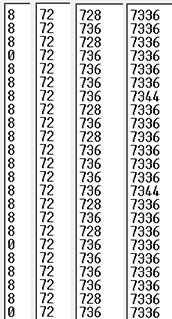
\includegraphics[scale=0.65]{MicroLab5/loops}}
\caption{Duration of program loop form 1000 to 1000000 repeats}
\end{figure}
The duration of one loop is $8ms/1000=8\mu s$.
\lstinputlisting[caption=main.c]{MicroLab5/main1.c}
\subsection{The second task}
I have modified my code for the second task:
\lstinputlisting[caption=L5\_12.c]{MicroLab5/L5_2.c}
\lstinputlisting[caption=L5\_12.h]{MicroLab5/L5_2.h}
\lstinputlisting[caption=main.c]{MicroLab5/main.c}
\subsection{The third task}
Not done.
\subsection{The fourth task}
We used the original L5\_12.c and L5\_12.h files from listings 1 and 2 for this task.\\\\
\lstinputlisting[caption=L5\_4.c]{MicroLab5/L5_4.c}
\subsection{The firth task}
We used the original L5\_12.c and L5\_12.h files from listings 1 and 2 for this task.
\lstinputlisting[caption=L5\_5.c]{MicroLab5/L5_5.c}



\end{document}
